\documentclass{article}
\usepackage[utf8]{inputenc}

\title{\textbf{Optimal low-thrust navigation around highly irregular asteroids with sequential convex programming}}
\author{Rory Lipkis, \textit{Stanford University, Department of Aeronautics and Astronautics}}
\date{}
\newcommand{\uvec}[1]{\boldsymbol{\hat{\textbf{#1}}}}
\newcommand{\conj}[1]{{#1}^{\dagger}}
\newcommand{\del}{\nabla}
\newcommand{\D}{\mathrm{d}}
\newcommand{\TD}[2]{\frac{d#1}{d#2}}
\newcommand{\TTD}[2]{\frac{d^{2}{#1}}{d{#2}^{2}}}
\newcommand{\PD}[2]{\frac{\partial#1}{\partial#2}}
\newcommand{\PPD}[2]{\frac{\partial^{2}{#1}}{\partial{#2}^{2}}}
\newcommand{\PPPD}[2]{\frac{\partial^{3}{#1}}{\partial{#2}^{3}}}
\newcommand{\la}{\langle}
\newcommand{\ra}{\rangle}
\newcommand{\const}[1]{\Big\rvert_{#1}}
\newcommand{\pfrac}[2]{\left(\frac{#1}{#2}\right)}
\usepackage{fullpage}
\usepackage{amsmath}
\usepackage{amssymb}
\usepackage{setspace}
\usepackage{mathtools}
\usepackage{enumerate}
\usepackage{esint}
\usepackage{booktabs}
\usepackage{physics}
\usepackage{siunitx}
\usepackage{graphicx}
\usepackage{graphics}
\usepackage{dsfont}
\usepackage{slashed}
\usepackage{multicol}
\usepackage{float}

\begin{document}

\maketitle

\abstract{The problem of low-thrust control around bilobate asteroids is explored with sequential convex programming. At each iteration, the gravitational dynamics as well as the collision inequality constraints are linearized around the solution from the previous iteration. The success of the approach is demonstrated with an example mission in which a spacecraft performs a soft landing on an asteroid, navigates across the surface, and returns to a mother ship.}

\noindent\rule{\linewidth}{1pt}

\begin{multicols}{2}
\section*{Introduction}
As interest in asteroid exploration missions increases, there is potential use for low-thrust control around irregularly-shaped gravitating bodies. Recent missions to asteroids 67P/Churyumov–Gerasimenko (Rosetta) and 486958 Arrokoth (New Horizons) revealed bilobate shapes, which appear to be a relatively common feature of asteroids (see Figure \ref{fig:67P}). These shapes, also known as \textit{contact binaries}, produce highly nonspherical gravitational potentials that cannot be easily navigated. 

\begin{figure}[H]
	\centering
	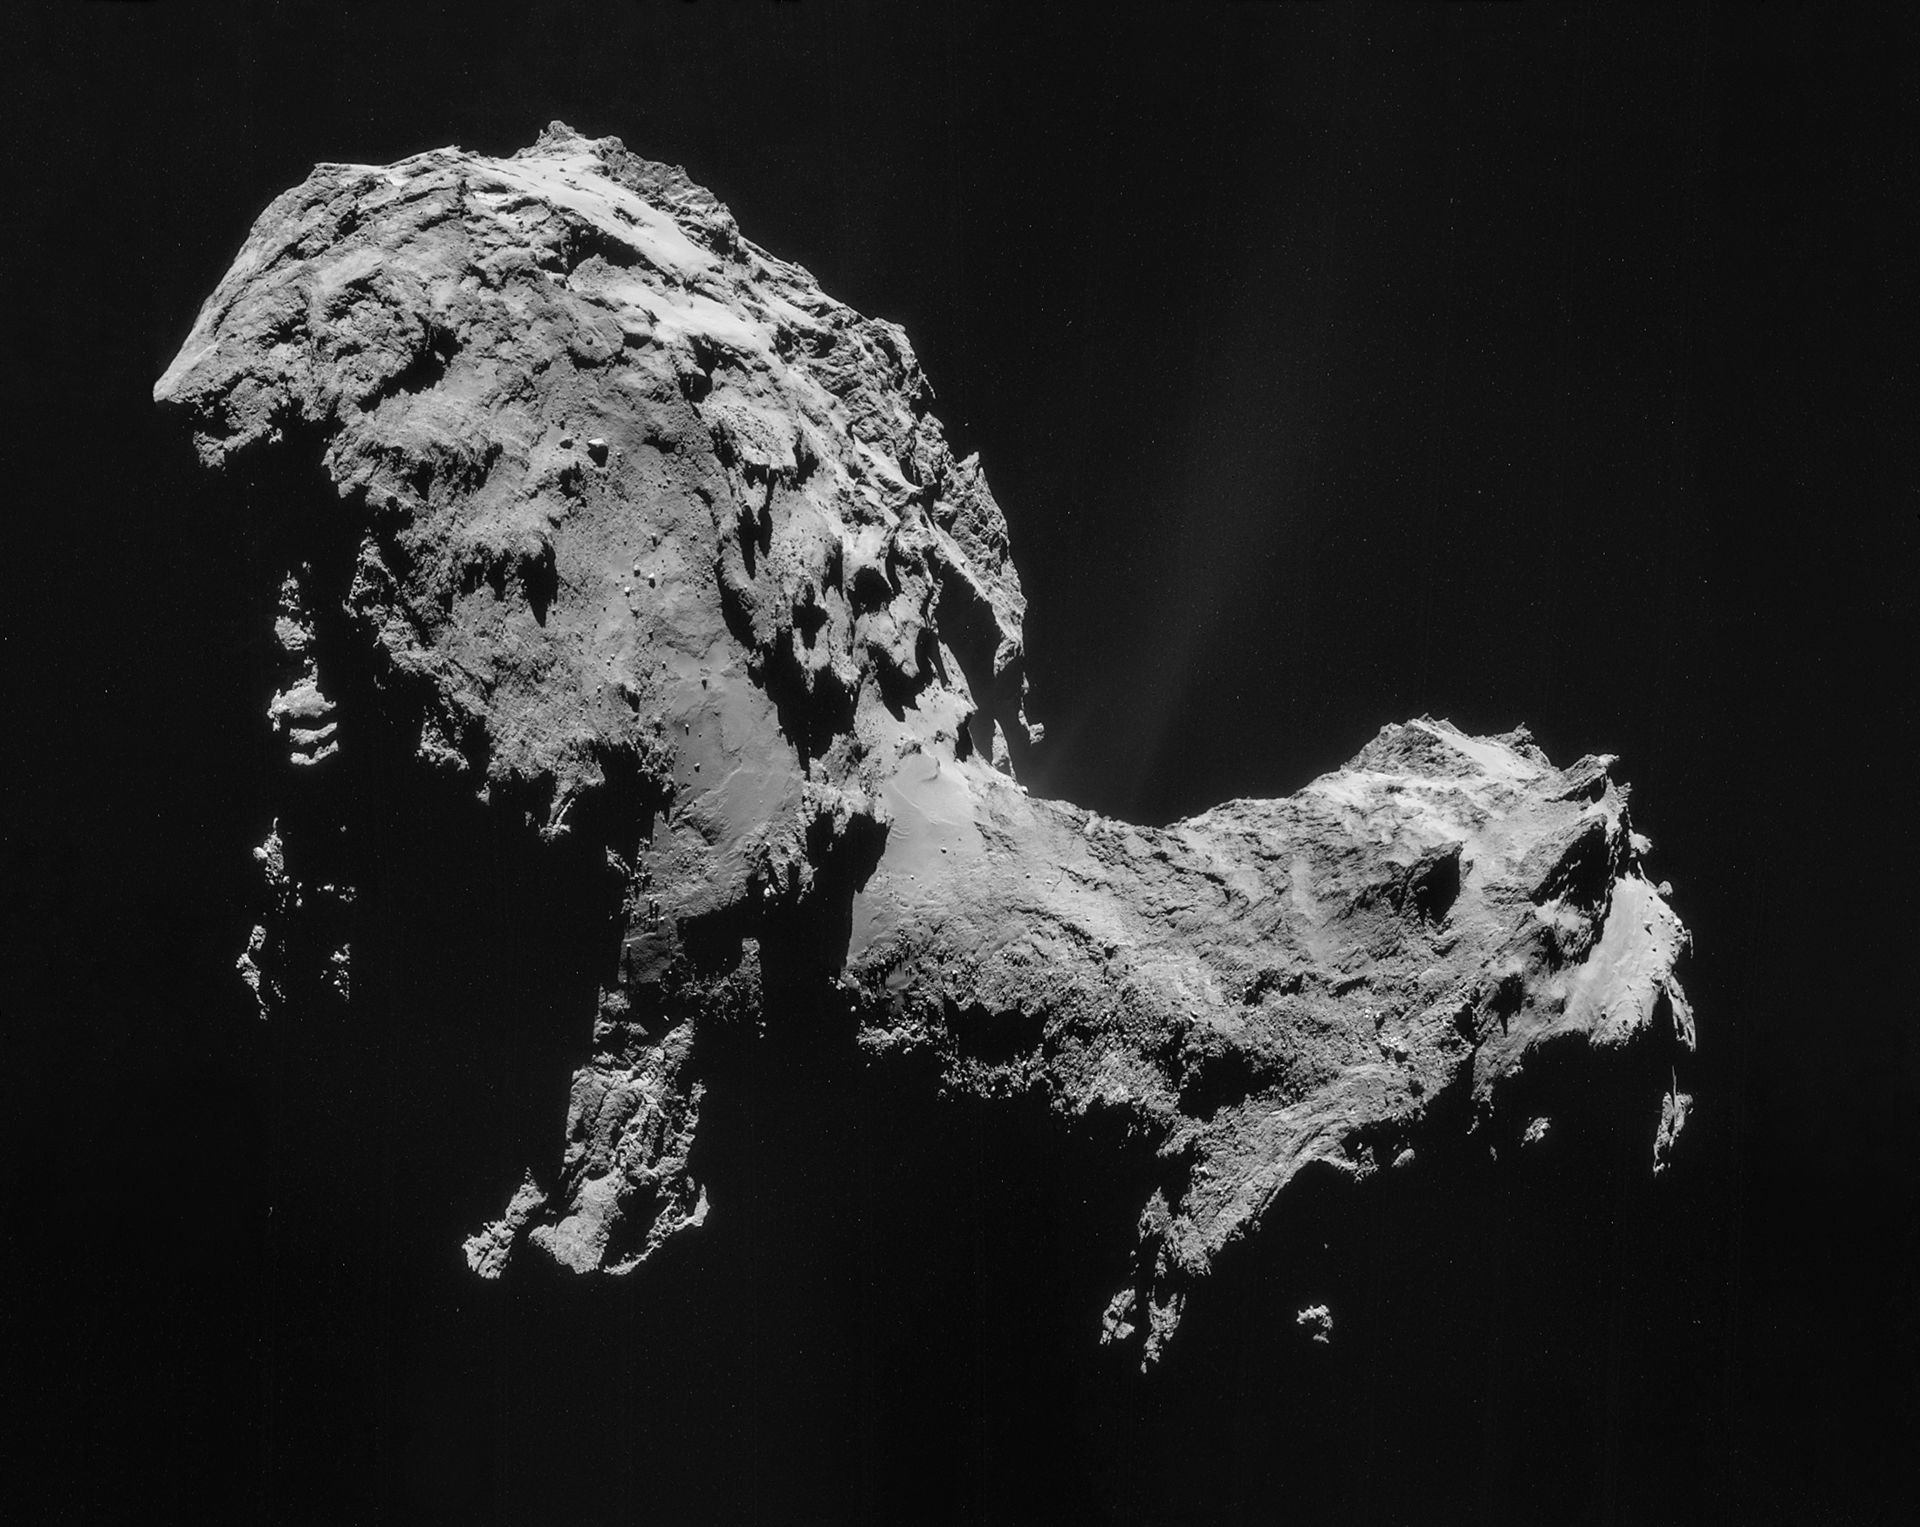
\includegraphics[width=0.8\linewidth]{figs/comet}
	\caption{Comet 67P, \textit{via Wikipedia}.}
	\label{fig:67P}
\end{figure}

Stacey and D'Amico 2018\footnote{Stacey, Nathan, and Simone D’Amico. ``Autonomous Swarming for Simultaneous Navigation and Asteroid Characterization.'' In \emph{AAS/AIAA Astrodynamics Specialist Conference}. 2018.} describe a method by which satellite formations could be used to perform initial estimation of asteroid gravitational fields. Although such gravitational fields must necessarily be very weak (or else the bodies would be pulled into spheroid), future missions that entail a large number of asteroid visits or independent spacecrafts must contend with potentially stringent thrust constraints, which limit the spacecraft control ability to within an order of magnitude of the surface gravity. In this domain, the irregularity of the gravitational becomes a nontrivial consideration.

Irregular gravitational fields are typically represented by their decomposition into spherical harmonics, the basis of Legendre polynomials. The standard orbital element representation of orbital motion can be modified to account for low-order harmonics, such as the $J2$ oblateness correction, with the introduction of mean and osculating elements, which specify an ``instantaneous'' unperturbed orbit. This extension allows control schemes that rely on orbital elements to be easily extended to find optimal thrust solutions around slightly oblate bodies. Though useful for orbits around planets, this method does not generalize to trajectories in highly irregular gravitational fields, whose specifications require extremely high order spherical harmonics, and where the notion of orbital elements ceases to be meaningful altogether. Since such trajectories are rarely stable orbits, and in fact are nearly always chaotic, they cannot be meaningfully specified by any set of periodic elements, and the Cartesian position and velocity state must be used instead.

\section*{Asteroid model}
This paper examines a simplified model of a bilobate asteroid, consisting of two spherical masses of constant density, each with radius $R_{i}$, oriented along an axis $\uvec{a}$. By modeling the asteroid in this way, the costly spherical harmonic representation is replaced by a direct Newtonian calculation, which allows for much higher ``orders'' to be effectively considered, despite the reduced detail. The graviational field of the asteroid is then given by
\begin{align*}
	\mathbf{f}_{g} = -\frac{GM_{1}(\mathbf{r} - \mathbf{r}_{1})}{|\mathbf{r} - \mathbf{r}_{1}|^{3}} - \frac{GM_{2}(\mathbf{r} - \mathbf{r}_{2})}{|\mathbf{r} - \mathbf{r}_{2}|^{3}}
\end{align*}
where
\begin{align*}
	\mathbf{r}_{1} &= \frac{m_{2}}{m_{1} + m_{2}}(R_{1} + R_{2})\uvec{a}\\
	\mathbf{r}_{2} &= -\frac{m_{1}}{m_{1} + m_{2}}(R_{1} + R_{2})\uvec{a}
\end{align*}
are the positions of the lobe centers in the center-of-mass frame.

\section*{Sequential convex programming}
The system is formalized by the state $\mathbf{s}$, formed by the concatenation of the spacecraft position and velocity. Along with the control input $\mathbf{u}$, the dynamics are written as
\begin{align*}
	\dot{\mathbf{s}} = \mathbf{f}(\mathbf{s}, \mathbf{u}) = 
	\begin{bmatrix}
	\mathbf{v}\\
	\mathbf{f}_{g} + \mathbf{u}
	\end{bmatrix}
\end{align*}
This is linearized around a reference state $\mathbf{s}_{0}$ and control input $\mathbf{u}_{0}$ by the first-order expansion
\begin{align*}
	\dot{\mathbf{s}} = \mathbf{f}(\mathbf{s}_{0}, \mathbf{u}_{0}) + A(\mathbf{s} - \mathbf{s}_{0}) + B(\mathbf{u} - \mathbf{u}_{0})
\end{align*}
The system matrix $A$ is given by
\begin{align*}
	A = \PD{\mathbf{f}}{\mathbf{s}}(\mathbf{s}_{0}, \mathbf{u}_{0}) =
	\begin{bmatrix}
	\mathbf{0}_{3\times3} & \mathbf{I}_{3\times3}\\
	A_{1} + A_{2} & \mathbf{0}_{3\times3}
	\end{bmatrix}
\end{align*}
where
\begin{align*}
	A_{i} = \frac{\mu(3\mathbf{d}_{i}\mathbf{d}_{i}^{T} - |\mathbf{d}_{i}|^{2}\mathbf{I}_{3\times3})}{|\mathbf{d}_{i}|^{5}}
\end{align*}
and $\mathbf{d}_{i} = \mathbf{r} - \mathbf{r}_{i}$ is the separation from a lobe center. The control matrix $B$ is given by
\begin{align*}
	B = \PD{\mathbf{f}}{\mathbf{u}}(\mathbf{s}_{0}, \mathbf{u}_{0}) = 
	\begin{bmatrix}
	\mathbf{0}_{3\times3}\\
	\mathbf{I}_{3\times3}
	\end{bmatrix}
\end{align*}
The sequential convex programming method solves at each iteration the problem
\begin{align*}
	\text{min} &\quad J(\mathbf{s}, \mathbf{u})\\
	\text{s.t.} &\quad \dot{\mathbf{s}}(t) = \mathbf{f}_{k}(\mathbf{s}(t), \mathbf{u}(t))\\
	&\quad \mathbf{s}(0) = \mathbf{s}_{0}\\
	&\quad \mathbf{u}(t) \in \mathcal{U}\\
	&\quad |\mathbf{s}(t) - \mathbf{s}_{k}(t)| \le \rho, \quad t \in [0,t_{f}]\\
\end{align*}
where $\mathbf{f}_{k}$ is the linearization of the dynamics with the previous solution trajectory $\mathbf{s}_{k}$ and control history $\mathbf{u}_{k}$ used as references. The dynamics constraint is enforced by an Euler integration that equates 
\begin{align*}
	\mathbf{s}_{t+1} = \mathbf{s}_{t} + \mathbf{f}_{k}(\mathbf{s}(t), \mathbf{u}(t))\Delta t
\end{align*}

% talk about modifications to cost, normalization, etc.
% show convergence plot

\section*{Implementation}
Several important considerations must be noted:

The equations of gravitational motion linearize notoriously poorly, and thus the trust region $\rho$ must be tuned to ensure convergence. Additionally, since neither the exact nor linearized dynamics admit a useful non-dimensional or similarity form, actual values for distance and mass must be used, resulting in extremely large costs that risk destabilizing the convex solver. The cost matrices must be carefully scaled to produce a cost of a reasonable order of magnitude.

This also necessitates that the cost be a function of the control history and the final state, but not the entire trajectory:
\begin{align*}
	J(\mathbf{s}, \mathbf{u}) = \mathbf{s}(t_{f})^{T}Q_{f}\mathbf{s}(t_{f}) + \int_{0}^{t_{f}} \mathbf{u}(t)^{T}R\mathbf{u}(t)\,dt
\end{align*}
The large distances involved at the beginning of an orbital ``regularization'' problem would otherwise result in large terms in the cost that completely overwhelm the control terms.

Explicitly forbidding the spacecraft trajectory from passing inside the asteroid is impossible, as it is a non-convex inequality constraint. Unfortunately, for many missions, especially ones in which the spacecraft begins close to the asteroid, the optimal trajectory found by the program is effectively a low-thrust Hohmann transfer, in which the spacecraft maneuvers as close to the bottom of the gravitational potential as possible, then expends as much thrust as possible at that point.\footnote{It can be shown that this sort of maneuver is generally optimal.} Without a collision constraint, the potentials go to $-\infty$ at the lobe centers. The addition of a ``penalty'' potential to discourage trajectories within the asteroid is problematic, since it adds a difficult non-differentiability to the system, which can cause the linearized problem to become incorrect or infeasible. 

The problem is solved by the linearization of the inequality constraint along with the dynamics. For each lobe, the true constraint is given by
\begin{align*} 
	|\mathbf{r} - \mathbf{r}_{i}| \ge R_{i}
\end{align*}

With all the necessary modifications made, the problem becomes feasible.

\section*{Example mission}
The utility of this method is demonstrated by a difficult mission in which a probe begins at a mother ship, descends into the furrow of an asteroid where the gravitational field is most nonlinear, performs a soft landing on the surface, maneuvers to another point on the asteroid in order to carry out various mission objectives, then returns to the mother ship. The lobes of the asteroid are $1\text{ km}$ and $2\text{ km}$ in radius, respectively, and the density is $2\text{ g/cm}^{3}$ uniformly. This results in a total mass of $7.54\times10^{13}\text{ kg}$. The low-thrust engines limit the control acceleration to $1\text{ cm/s}^{2}$.

The descent is optimized by choosing an initial control history of zero magnitude. The state and control histories are plotted in Figure \ref{fig:desc_plots}, and the full trajectory is displayed in Figure \ref{fig:desc_traj}.

\begin{figure}[H]
	\center
	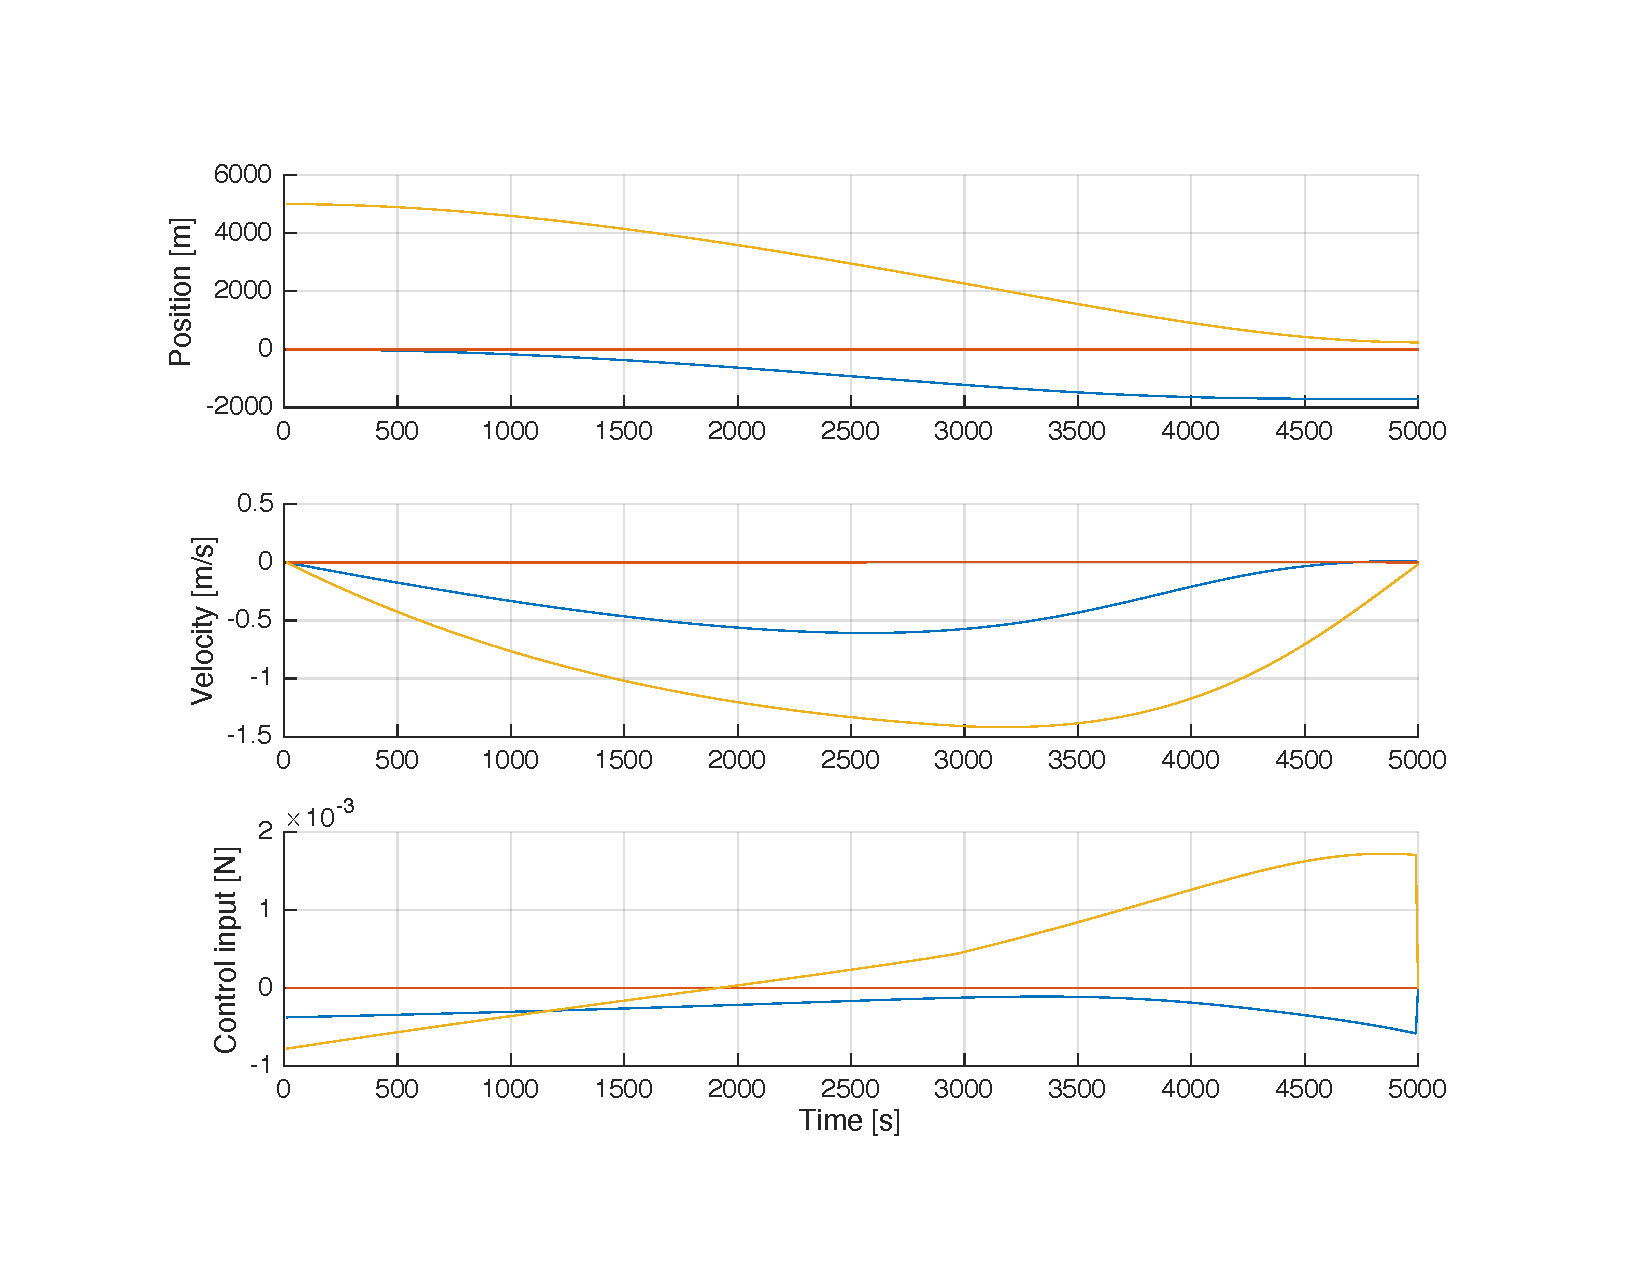
\includegraphics[width=0.85\linewidth]{figs/desc_plots}
	\caption{Position components, velocity components, and control components for descent.}
	\label{fig:desc_plots}
\end{figure}

\begin{figure}[H]
	\center
	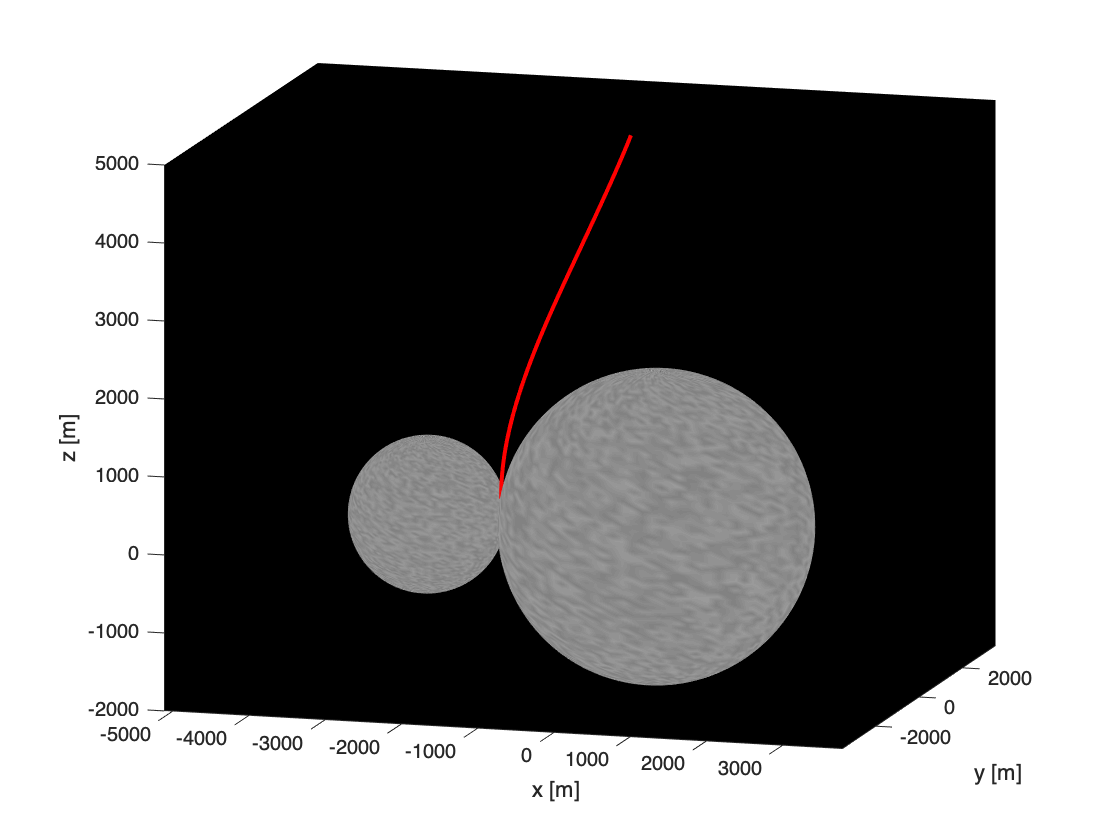
\includegraphics[width=0.85\linewidth]{figs/desc_traj}
	\caption{Trajectory of descent.}
	\label{fig:desc_traj}
\end{figure}

The ascent is somewhat more difficult. Because of the initial closeness to the asteroid, the initial controls must be chosen with some care to enable proper convergence: a uniform upwards thrust suffices. The state and control histories are plotted in Figure \ref{fig:asc_plots}, and the full trajectory is displayed in Figure \ref{fig:asc_traj}. Note its similarity to the time of the descent state and control histories: this symmetry is a good indication of the program's robustness. 

\begin{figure}[H]
	\center
	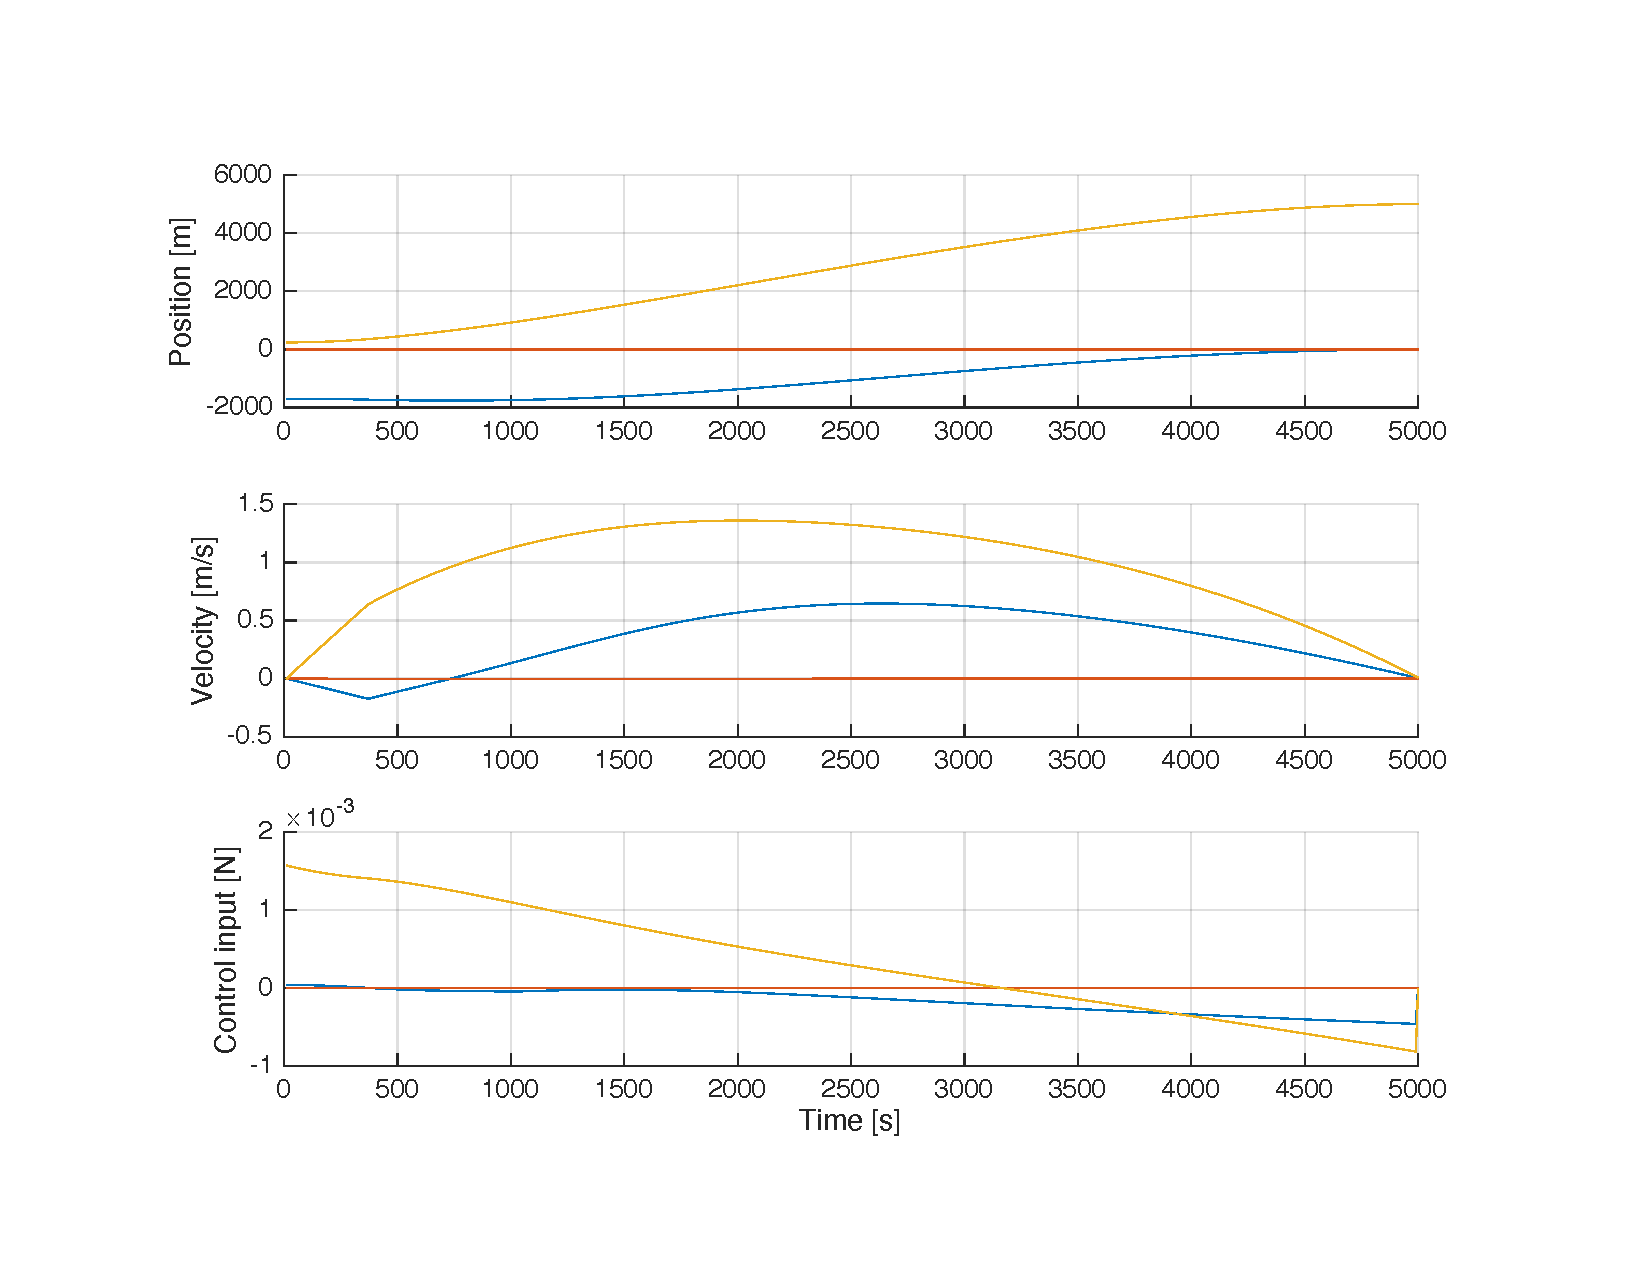
\includegraphics[width=0.85\linewidth]{figs/asc_plots_good}
	\caption{Position components, velocity components, and control components for ascent.}
	\label{fig:asc_plots}
\end{figure}

\begin{figure}[H]
	\center
	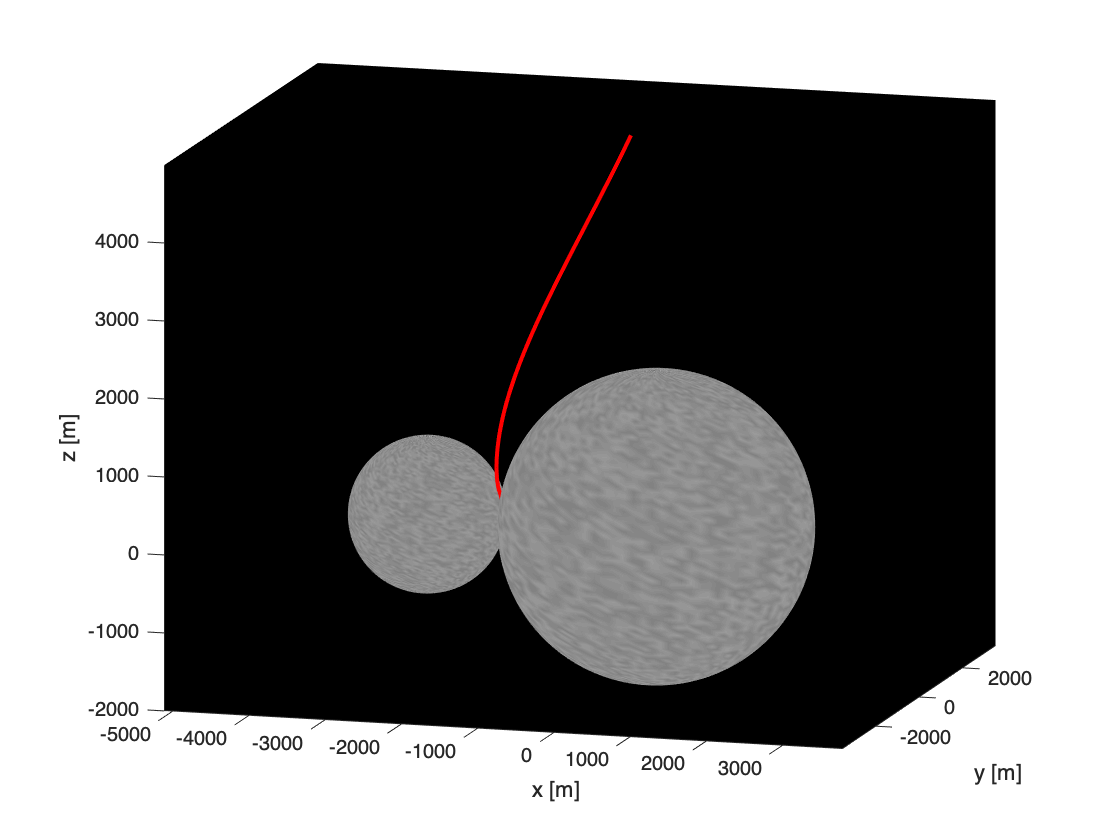
\includegraphics[width=0.85\linewidth]{figs/asc_traj_good}
	\caption{Trajectory of ascent.}
	\label{fig:asc_traj}
\end{figure}

\section*{Discussion}
A major source of error in the solutions is the inaccuracy of the Euler integration. Experiments were performed with high-order integration schemes and linear multi-step methods, such as the Adams-Moulton method, which is known to perform well for orbital determination due to its stability and accuracy. Although the trajectories produced are closer to the true integrated solutions, the increased complexity can be destabilizing. However, this is a promising area for future development of this problem. 

Future work would also account explicitly for asteroid rotation -- currently, the effect can be captured by mandating that the final state contain some pre-calculated tangential velocity.

The largest area for future work is the collision potential. Possibly a barrier potential

Convergence is still not guaranteed because of high costs.

\section*{Acknowledgments}
The author would like to thank Prof. Pavone and the AA203 teaching staff.

\end{multicols}
\end{document}